The Standard Model of particle physics is one of the most precisely tested
theories. It is a relatistivic quantum field theory using the Lagrange
formalism.

It provides a unified description of three of the four forces of nature: the
electromagnetic interaction, the weak interaction, and the strong
interaction. Gravitation not included.

Natural units $\hbar = c = 1$. Can be recovered by dimensional
analysis. Heaviside--Lorentz units?

Einstein summation convention: Sum over repeated indices.

Space-time indices are given as greek letters. All other indices are latin.

Cross-sections in barn $\SI{1}{\barn} = 10^{-28}\,\si{\metre\squared}$

Cite what this description is based on: \cite{Halzen:1984mc,Thomson:2013zua}


\section{Particles and Interactions in the Standard Model}

The Standard Model, shown in~\Cref{fig:sm_particles}, consists of 12 elementary
spin-$\frac{1}{2}$ particles referred to as \emph{fermions} and their
anti-particles, and five types of particles with integer spin referred to as
\emph{bosons}. With the discovery of the Higgs boson in
2012~\cite{HIGG-2012-27,CMS-HIG-12-028}, experimental evidence for the existence
of all fermions and bosons predicted by the Standard Model is established.

\begin{figure}[htbp]
  \centering

  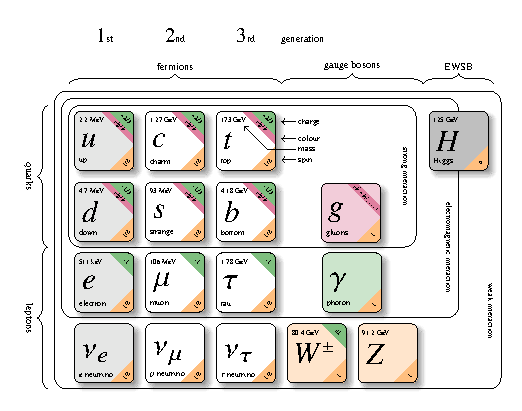
\includegraphics[width=\textwidth]{theory/sm}

  \caption{Particles of the SM. The diagram is adapted from Ref.~\cite{sm_tikz}
    with updated particle properties from Ref.~X. Antiparticles are not shown
    explicitly have additive quantum numbers of opposite sign but otherwise the
    same properties of the respective particle.}
  \label{fig:sm_particles}
\end{figure}


The elementary particles of the SM can be divided into three categories:
\begin{description}

\item[Fermions] predicted by the SM have spin-$\frac{1}{2}$. Consequently, they
  are massive\footnote{Neutrinos are considered as massless in the SM, however,
    the observation of neutrino
    oscillations~\cite{Super-Kamiokande:1998kpq,SNO:2002tuh} is experimental
    evidence for neutrinos having small but non-zero mass.} and adhere to the
  Pauli exclusion principle and are therefore considered to be \emph{matter}
  particles. For every fermions, a corresponding anti-particle exists that has
  the same properties but with opposite additive quantum numbers. The fermions
  of the SM are divided into \emph{quarks} that take part in the strong
  interaction and \emph{leptons} that do not. They are further divided into
  up-type quarks ($u$, $c$, $t$), down-type quarks ($d$, $s$, $b$), charged
  leptons ($e$, $\mu$, $\tau$), and neutrinos ($\nu_e$, $\nu_\mu$,
  $\nu_\tau$). The fermions of the SM come in three generations, the main
  difference between them being the mass of the fermions. All ordinary (stable)
  matter consists of fermions of the first generation: up-quarks, down-quarks,
  and electrons.

  The fermions carry charge-like quantum numbers that dictate the fundamental
  interactions they take part in. Quarks carry \emph{colour charge} which comes
  in three discrete values of either \emph{red}, \emph{green}, or \emph{blue},
  and the corresponding anti-colours for anti-quarks. Particles carrying colour
  charge take part in the strong interaction. Quarks and (electrically) charged
  leptons carry \emph{electric charge} and are therefore subject of the
  electromagnetic interaction. Fermions (anti-fermions) with left-handed
  (right-handed) chirality carry \emph{weak isospin} therefore taking part in
  charged-current weak interactions. All fermions carry \emph{weak hypercharge}
  and therefore take part in neutral current weak interactions.

\item[Gauge bosons] predicted by the SM are particles with spin-$1$ and are
  therefore also referred to as vector bosons. Gauge bosons are the quanta of
  fields arising in theories built on certain symmetry principles, referred to
  as gauge theories, which will discussed in
  \Cref{sec:theo_symmetries_interactions}. The gauge bosons mediate the three
  fundamental forces of nature through particle exchange.

  The (massless) gluons mediate the strong interaction through exchange of
  gluons between particles carrying colour charge. Gluons carry colour charge
  themselves and therefore couple to quarks or other gluons. The (massless)
  photon mediates the electromagnetic interaction between electrically charged
  particles. The gauge bosons of the weak interaction, the $W^\pm$ and $Z$
  bosons, take a special role in the SM since they are the only massive gauge
  bosons. The $W$ bosons are electrically charged and mediate the charged
  current weak interaction between particles carrying weak isospin. The
  uncharged $Z$ boson mediates the neutral-current weak interaction between
  particles carrying weak hypercharge.

\item[The Higgs boson] is the only scalar (spin-$0$) particle in the SM. The
  Higgs boson is a by-product of the Brout--Englert--Higgs (BEH)
  mechanism~\cite{Englert:1964et,Higgs:1964pj} that is used to include massive
  gauge bosons, the $W^\pm$ and $Z$ bosons, in the SM without violating the
  underlying principles of the gauge theory. This will be elaborated in
  \Cref{todo}.

\end{description}


\section{Symmetries and Interactions}
\label{sec:theo_symmetries_interactions}

% \subsection{The Langrange Formalism}

The SM is a relativistic quantum field theory and thus described by space-time
dependent fields $\phi_i(\myvec{x})$. The dynamics of fields are given by the
\emph{Lagrangian density}, $\lagrange$, which is a function of the fields
$\phi_i$ and their space-time derivatives
$\partial_\mu \phi_i = \partial \phi_i / \partial x^\mu$ ($\mu = 0, 1, 2,
3$). The time-evolution of the fields follows from the principle of least
action, i.e.\ by minimising the action
$S = \int \mathrm{d}^4x \, \lagrange(\phi_i, \partial_\mu \phi_i)$, which yields
the the Euler--Lagrange equations
\begin{align*}
  \partial_{\mu} \left( \frac{\partial \lagrange}{\partial (\partial_{\mu} \phi_i)} \right) - \frac{\partial \lagrange}{\partial \phi_i} = 0
\end{align*} that provide the equations of motion for the fields. The Lagrangian density is
hereafter referred to as \emph{the Lagrangian}.

% \subsection{Local Gauge Invariance}

A continuous transformation of the fields that leaves the Lagrangian unchanged
is referred to as a \emph{gauge transformation}. The fields resulting from this
transformation follow the same equations of motion and thus describe the same
physical system. This invariance is referred to as \emph{gauge invariance} or
\emph{gauge symmetry}.
% An external observer cannot distinguish between fields related by gauge
% transformations and therefore the symmetry is considered an \emph{internal
% symmetry} of the theory.
The symmetry groups relevant for the description of the SM are the unitary group
of dimension one, $U(1)$, and the special unitary groups of dimension two and
three, $SU(2)$ and $SU(3)$, respectively. Any element of a unitary or special
unitary group can be written as
\begin{align*}
  \hat{U} = \exp\big[ i \theta_a G^a \big] \,\text{,}
\end{align*}
where $\theta_a$ are real parameters, $G^a$ are the generators of the group, and
summation over repeated indices is implied. A Lagrangian that is invariant to a
transformation $\hat{U}$ of the fields with parameters $\theta_a$ is said to
possess \emph{global} gauge invariance. The more restrictive case where the
Lagrangian is invariant with respect to transformations of the fields with
space-time dependent parameters $\theta_a(\myvec{x})$ is referred to as
\emph{local} gauge invariance.

This is illustrated in the case of the Lagrangian of the Dirac field of mass $m$
given by
\begin{align}
  \lagrange_{\text{Dirac}} = \bar{\psi} (i \gamma^\mu  \partial_\mu - m) \psi \,\text{,}
  \label{eq:dirac_lagrangian}
\end{align}
where $\psi$ ($\bar{\psi} = \psi^\dagger \gamma^0$) are (adjoint) Dirac spinors,
and $\gamma^\mu$ are the four Dirac matrices. \Cref{eq:dirac_lagrangian}
possesses global gauge invariance with respect to transformations from the
$U(1)$ group given by $\psi \to \psi^\prime = \exp[ i q \theta ] \psi$, where
$q$ is a coupling constant. However, when performing a local transformation
according to $\psi \to \psi^\prime = \exp[ i q \theta(\myvec{x}) ] \psi$ the
invariance of the Lagrangian is spoiled due to the derivative acting on the
space-time dependent phase factor. One might impose $U(1)$ local gauge
invariance of the Lagrangian by adding terms to \Cref{eq:dirac_lagrangian} that
cancel the additional contributions. Conventionally, this is done by
substituting the derivative $\partial_\mu$ by a gauge covariant derivative
$D_\mu$ that transforms as
$D_\mu\psi \to \exp[ i q \theta(\myvec{x}) ] D_\mu\psi$ thus recovering local
gauge invariance. The definition of $D_\mu$ with these properties requires the
introduction of a new massless vector field, referred to as a \emph{gauge
  field}, with appropriate transformation properties:
\begin{align}
  D_\mu = \partial_\mu + i q A_\mu \qquad \text{with} \qquad A_\mu \xrightarrow{U(1)} A_\mu^\prime = A_\mu - \partial_\mu \theta(\myvec{x}) \,\text{.}
  \label{eq:covariant_derivative_qed}
\end{align}
The additional term introduced by substituting $\partial_\mu \to D_\mu$ in
\Cref{eq:dirac_lagrangian} is interpreted as an interaction between the fermion
and the vector boson of the gauge field.

The principle of local gauge invariance can be used to obtain the Lagrangian of
quantum electrodynamics (QED) describing electromagnetic interactions. The
symmetry group of QED is $U(1)_{Q}$, the subscript $Q$ indicating that the
elements of this group act on fields with electric charge. Imposing local gauge
invariance by substituting \Cref{eq:covariant_derivative_qed} into the Dirac
Lagrangian yields the interaction term
\begin{align*}
  \lagrange_{\text{int}} = - q \bar{\psi} \gamma^\mu \psi A_\mu \,\text{.}
\end{align*}
In the case of QED, the field $A^\mu$ is identified as the four-potential of the
electromagnetic field, and the coupling constant $q$ as the charge of the
fermion. Therefore, $\lagrange_{\text{int}}$ describes the coupling between the
photon and a fermion with electric charge $q$. For a single fermion type, the
Lagrangian of QED is given by
\begin{align*}
  \lagrange_{\text{QED}} = \underbrace{\lagrange_{\text{Dirac}}}_{\text{Free fermion field}}
  \quad\underbrace{- q \bar{\psi} \gamma^\mu \psi A_\mu}_{\text{Fermion--photon interaction}}
  \quad\underbrace{- \frac{1}{4} F_{\mu\nu} F^{\mu\nu}}_{\text{Free photon field}} \,\text{,}
\end{align*}
which additionally includes the Lagrangian of the free photon field defined by
the electromagnetic tensor given by
$F_{\mu\nu} = \partial_\mu A_\nu - \partial_\nu A_\mu$. The additional term also
fulfils the local gauge invariance with respect to $U(1)_Q$.

The theoretical description of the SM heavily relies on the principle of local
gauge invariance outlined previously. The symmetry group of the SM is
\begin{align*}
  SU(3)_{\text{color}} \otimes SU(2)_{\text{L}} \otimes U(1)_Y \,\text{,}
\end{align*}
where $SU(3)_{\text{color}}$ is the symmetry of the strong interaction, and
$SU(2)_{\text{L}} \otimes U(1)_Y$ the symmetry of the unified description of the
electromagnetic and weak interaction. These will be introduced in
\Cref{sec:theory_qcd} and \Cref{seq:theory_ewk}, respectively.

% \todo[inline]{Maybe note that a mass term a la $\frac{1}{2} m^2 A_\mu A^\mu$
%   would violate local gauge invariance.}

% \todo[inline]{Concluding remarks???}


\subsection{Quantum Chromodynamics}%
\label{sec:theory_qcd}

Quantum chromodynamics (QCD) is the quantum field theory describing the
interactions of quarks and gluons. The fundamental charge of QCD is colour
charge which comes in three distinct colors referred to as red, green, and blue
(r, g, b). The quark fields are consequently written in terms of the three
component objects
\begin{align*}
  \psi =
  \begin{pmatrix}
    q_\text{r} \\
    q_\text{g} \\
    q_\text{b}
  \end{pmatrix}
  \qquad
  \text{and}
  \qquad
  \bar{\psi} =
  \begin{pmatrix}
    \bar{q}_\text{r} & \bar{q}_\text{g} & \bar{q}_\text{b}
  \end{pmatrix} \,\text{,}
\end{align*}
in which the $q_i$ ($\bar{q}_i$) represent (adjoint) Dirac spinors describing
the quark field with color $i$. The strong interaction does not distinguish
between quarks of different colour thus assigning a $SU(3)_{\text{colour}}$
symmetry group to QCD, the subscript indicating that elements of the group act
in colour-space. The generators of $SU(3)_{\text{colour}}$ are taken to be
\begin{align*}
  T_a = \frac{1}{2} \lambda_a \qquad \text{for} \qquad a = 1, \dots, 8 \,\text{,}
\end{align*}
where $\lambda_a$ are the Gell-Mann matrices.\footnote{Latin indices are raised
  and lowered according to $T_a = \delta_{ab} T^b$ or $T^a = \delta^{ab} T_b$,
  where $\delta$ refers to the Kronecker delta and the Einstein summation
  convention is adopted.} The theory of QCD is referred to as a Yang--Mills
gauge theory~\cite{Yang:1954ek} since the elements of $SU(3)_{\text{colour}}$ do
not commute in general, i.e.\ the group is non-Abelian. The commutation relation
between the generators is given by $[T_a, T_b] = i f_{abc} T^c$, defining the
structure constants $f_{abc}$ of the group.

Following the principle of local gauge invariance regarding a local
$SU(3)_{\text{color}}$ transformation
\begin{align*}
  \psi \to \psi^\prime = \exp[ i g_{\text{s}} \theta_a(\myvec{x}) T^a] \psi
  &&\bar{\psi} \to \bar{\psi}^\prime = \bar{\psi} \exp[ - i g_{\text{s}} \theta_a(\myvec{x}) T^a]  \,\text{,}
\end{align*}
where $g_{\text{s}}$ is referred to as the strong coupling constant, yields the
covariant derivative and eight massless gauge fields $G_\mu^a$
\begin{align*}
  D_\mu = \partial_\mu + i g_{\text{s}} G_\mu^a T_a
  \qquad \text{with} \qquad
  G_\mu^k \xrightarrow{SU(3)_{\text{colour}}} {G_\mu^k}^\prime = G_\mu^k  - \partial_\mu \theta^k(\myvec{x}) - g_{\text{s}} f_{ijk} \theta^i(\myvec{x}) G_\mu^j \,\text{.}
\end{align*}
The gauge invariant kinetic term for the gluon fields is given by
\begin{align*}
  \lagrange_{G} = - \frac{1}{4} G_{\mu\nu}^{a} G^{\mu\nu}_{a}
\end{align*}
with the gluon field strength tensor
\begin{align*}
  G_{\mu\nu}^i = \partial_\mu G_\nu^i - \partial_\nu G_\mu^i - g_{\text{s}} {f^{i}}_{jk} G_\mu^j G_\nu ^k \,\text{.}
\end{align*}
The Lagrangian of QCD for a single flavour of quark with mass $m$ is
consequently given by
\begin{align}
  \lagrange_{\text{QCD}} =
  \underbrace{\bar{\psi} (i \gamma^\mu \partial_\mu - m) \psi}_{\text{Free quark field}}
  \underbrace{- g_{\text{s}} (\bar{\psi} \gamma^\mu T_a \psi) G_\mu^a}_{\text{Quark--gluon interactions}}
  \underbrace{- \frac{1}{4} G_{\mu\nu}^a G^{\mu\nu}_a}_{\text{Kinetic term}} \,\text{.}
  \label{eq:qcd_lagrangian}
\end{align}
This Lagrangian describes the free quark field, the interactions of quarks with
the eight gluons, and the kinetic energy contained in the gluon fields (the
kinetic term). The non-Abelian nature of the $SU(3)_{\text{colour}}$ group,
meaning a set of indices exists such that $f_{abc} \neq 0$, gives rise to the
distinct structure of QCD through the kinetic terms of the gluon fields in the
Lagrangian. These terms include self-interactions between gluons which
correspond to, in the language of Feynman diagrams, to triple and quartic gluon
vertices. Gluons themselves are carriers of colour charge which ultimately lead
to such behaviour. This is unlike the photon of QED which does not carry any
electrical charge and therefore does not couple to itself.

A number of features originate from the theory of QCD which are enumerated in
the following:
\begin{description}

\item[Colour confinement] Due to the dynamics of the gluon self-interactions,
  free quarks or gluons cannot be observed in nature. Separating the quarks of a
  quark--antiquark pair leads to the formation of \emph{flux tubes} in the gluon
  field strength that result in a linear increase in field energy with
  separation of the quarks. Eventually, the energy stored in the gluon field is
  sufficiently large to create a quark--antiquark pair from the
  vacuum. Ultimately, only quarks (or gluons) bound into colourless composite
  particles (colour singlett states) remain. The most prevalent bound states of
  quarks are (anti-)baryons consisting of three (anti-)quarks, and mesons
  consisting of a quark--antiquark pair. The $SU(3)_{\text{colour}}$ symmetry
  also allows for colour singlett states of multiple gluons referred to as
  \emph{glueballs}, or other combinations of quarks such as tetra-
  ($q_1 \bar{q}_2 q_3 \bar{q}_4$) or pentaquarks ($q_1 q_2 q_3 q_4 \bar{q}_5$).

\item[Asymptotic freedom]

\end{description}


\subsection{Theory of the Electroweak Interaction}%
\label{seq:theory_ewk}

The theory of the electroweak interaction was developed by Glashow, Salam, and
Weinberg in the 1960s unify the electromagnetic and weak interaction in a single
model~\cite{Glashow:1961tr,Salam:1964ry,Weinberg:1967tq}. The model is based on
the requirement of gauge invariance under $SU(2)_{\text{L}} \times U(1)_{Y}$,
where



The weak interaction via charged currents violates parity
conservation~\cite{Wu:1957my} maximally by only coupling to particles with
left-handed and anti-particles with right-handed chirality. This suggests, that
the charged-current weak interaction adheres to a $SU(2)$ symmetry


neutral current that does not change the flavour of the particle.

Eigenstates of the charged-current weak interaction are indicated as
$\{ d^\prime, s^\prime, b^\prime \}$ to differentiate them from the eigenstates
of the strong interaction $\{ d, s, b \}$. The relationship between these
representations is given by the Cabibbo--Kobayashi--Maskawa matrix.

$SU(2)_{\text{L}}$

Neutrino scattering experiments show that the neutral current is not purely
left-handed.


Weak isospin $I$ quantised along an arbitrary third axis yielding the $I_3$
quantum numbers.


Doublet under $SU(2)_{\text{L}}$ left-handed chiral particles
\begin{align*}
  \begin{pmatrix}
    u \\
    d^\prime
  \end{pmatrix}_{\text{L}}
  \quad
  \begin{pmatrix}
    \nu_\ell \\
    \ell^{-}
  \end{pmatrix}_{\text{L}}
\end{align*}


GSW model unifying the electromagnetic and weak interactions.



charged-current interaction $SU(2)$ symmetry -> weak isospin

Left handed chiral particles are in a weak isospin doublet

Right handed chiral particles are in a weak isospin singlett

Vice versa for antiparticles


Gell-Mann--Nishijima:
\begin{align*}
  Y = 2 (Q  - I_3)
\end{align*}


\begin{align*}
  \begin{pmatrix}
    A_\mu \\
    Z_\mu
  \end{pmatrix}
  =
  \begin{pmatrix}
    \cos\theta_{\text{W}} & \sin\theta_{\text{W}} \\
    -\sin\theta_{\text{W}} & \cos\theta_{\text{W}}
  \end{pmatrix}
  \begin{pmatrix}
    B_\mu \\
    W_\mu^3
  \end{pmatrix}
\end{align*}


The coupling constant of the weak interaction is closely related to the coupling
constant of QED:
\begin{align*}
  e = g_{\text{W}} \sin\theta_{\text{W}}
\end{align*}

\section{Electroweak Symmetry Breaking}

\section{Fermion Masses}

\section{The Higgs Boson}


\clearpage

%%% Local Variables:
%%% mode: latex
%%% TeX-master: "../../phd_thesis"
%%% End:
